%%%%%%%%%%%%%%%%%%%%%%%%%%%%%%%%%%%%%%%%%
% Sleek, Extensible Journal Article
% LaTeX Template
% Version 0.1
% Date 01/05/2014
%
% Original author:
% Calem Bendell
%
% License:
% CC BY-NC-SA 3.0 (http://creativecommons.org/licenses/by-nc-sa/3.0/)
%
%%%%%%%%%%%%%%%%%%%%%%%%%%%%%%%%%%%%%%%%%

\documentclass[paper=128mm:96mm, fontsize=11pt, pagesize]{scrartcl}

\linespread{1.12}

\usepackage{soul}
\usepackage[default]{cabin}
\linespread{1.05}
\usepackage{microtype}

\setlength{\parskip}{0pt}

\usepackage[hang, small,labelfont=bf,up,textfont=it,up]{caption}
\usepackage[hidelinks, colorlinks=true]{hyperref}
\usepackage{booktabs, float, paralist, abstract, titling, enumitem, graphicx}
\usepackage[compact]{titlesec}
\usepackage[usenames,dvipsnames,svgnames,table]{xcolor}
\usepackage[flushmargin,hang,multiple]{footmisc}
\interfootnotelinepenalty=10000

\usepackage[top=4em, bottom=4em, left=3em, right=3em]{geometry}

\renewcommand{\abstractnamefont}{\normalfont\large\sffamily}
\renewcommand{\abstracttextfont}{\normalfont\itshape}

\titleformat{\section}
  {\normalfont\LARGE}{}{0pt}{\LARGE}
\titleformat*{\subsection}{\large\sffamily}
\titleformat*{\subsubsection}{\itshape\sffamily}
\titleformat*{\paragraph}{\large\bfseries\sffamily}
\titleformat*{\subparagraph}{\large\bfseries\sffamily}

\setlist[description]{format=\normalfont\itshape}

\renewcommand{\maketitle}{\noindent\rule{\linewidth}{1pt}\Huge \vspace{1em} \newline
\sffamily \scshape \thetitle \\
\normalfont \sffamily  \theauthor \\
\thedate
\newline\noindent\rule{\linewidth}{1pt}
\normalfont
\normalsize}

\pagestyle{empty}


\title{Computer Science \\ Undergraduate Society \vspace*{1em}}
\author{
\large
CSUS, McGill University \\
\normalsize \href{mailto:csus@cs.mcgill.ca}{csus@cs.mcgill.ca} \\
a copy of this presentation available at: mcgill-csus.github.io
}
\date{}

\begin{document}

\maketitle

\clearpage

	\begin{center}
	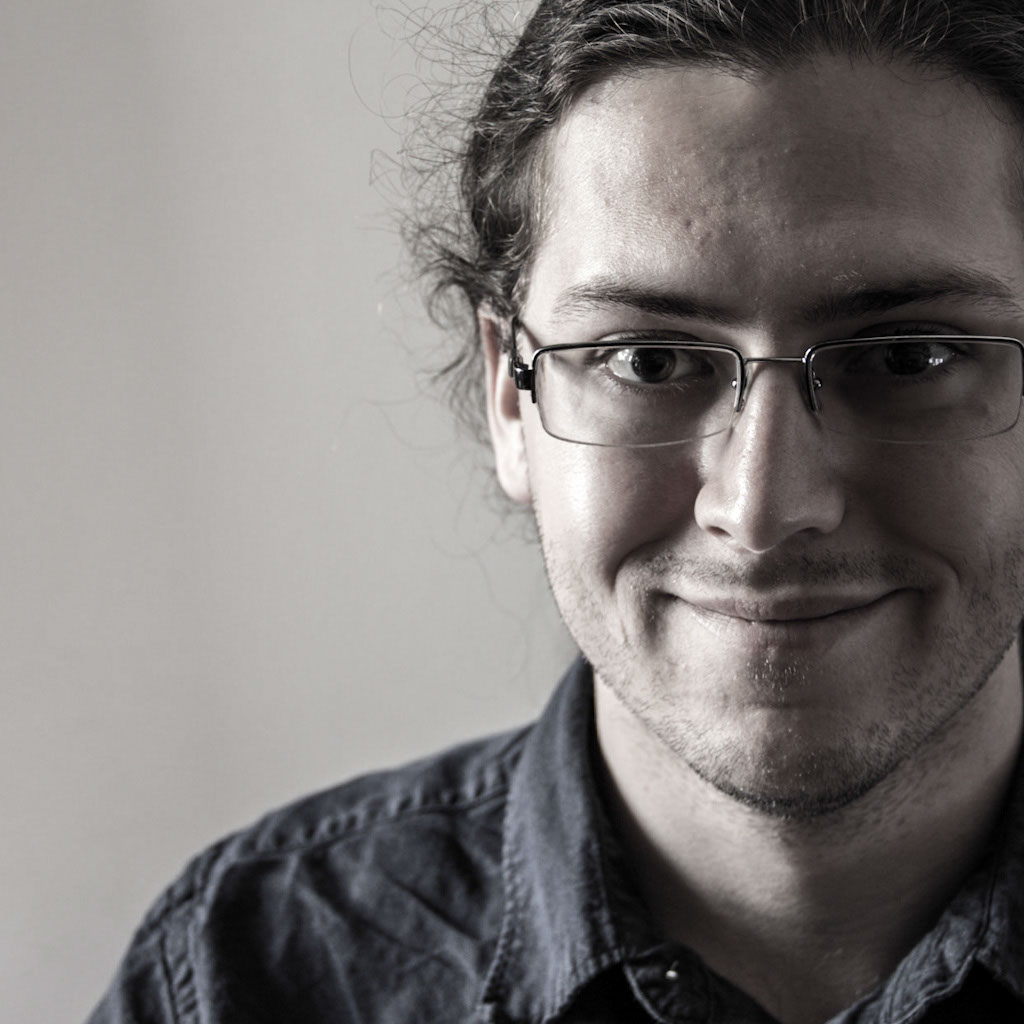
\includegraphics[width=.35\textheight]{gfx/calbenthumbsmall.jpg}
	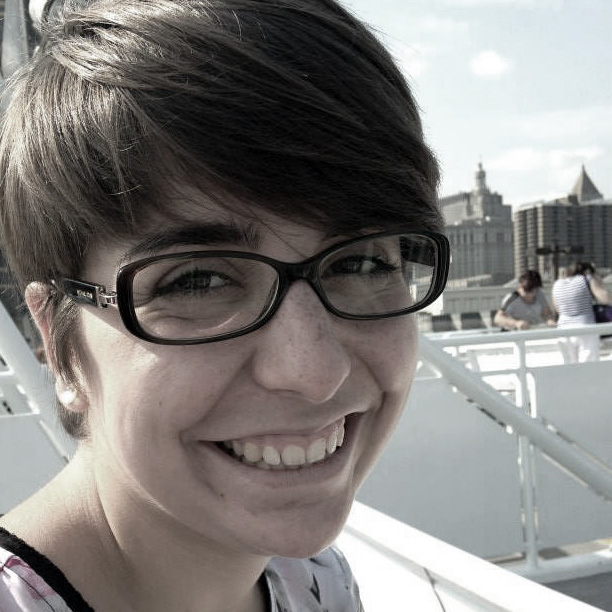
\includegraphics[width=.35\textheight]{gfx/maudethumb.jpg}
	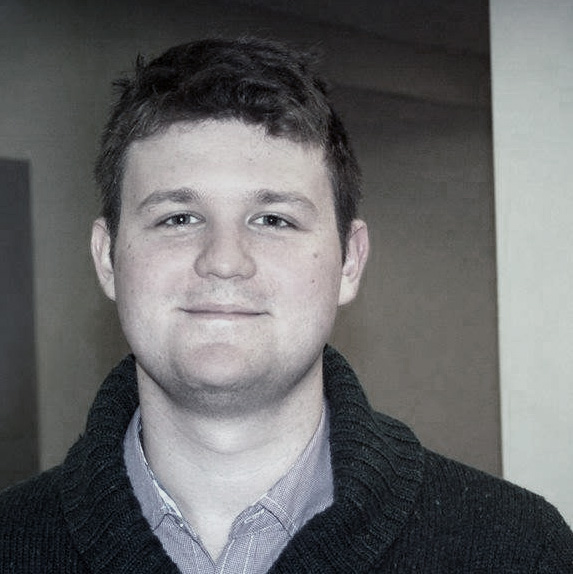
\includegraphics[width=.35\textheight]{gfx/maximthumb.jpg}
	\vspace{.5em}\newline
	 	\begin{tabular}{r|c|l}
	 		President - Calem & Academics - Maude & External - Maxim\\ \hline
	 		Internal - Zi Li & Admin - Saige & Finance - Genevieve\\ 
	 		
	 	\end{tabular}
	 	\vspace{.5em}\newline
	 	
\includegraphics[width=.35\textheight]{gfx/zilithumbsmall.jpg}
	 	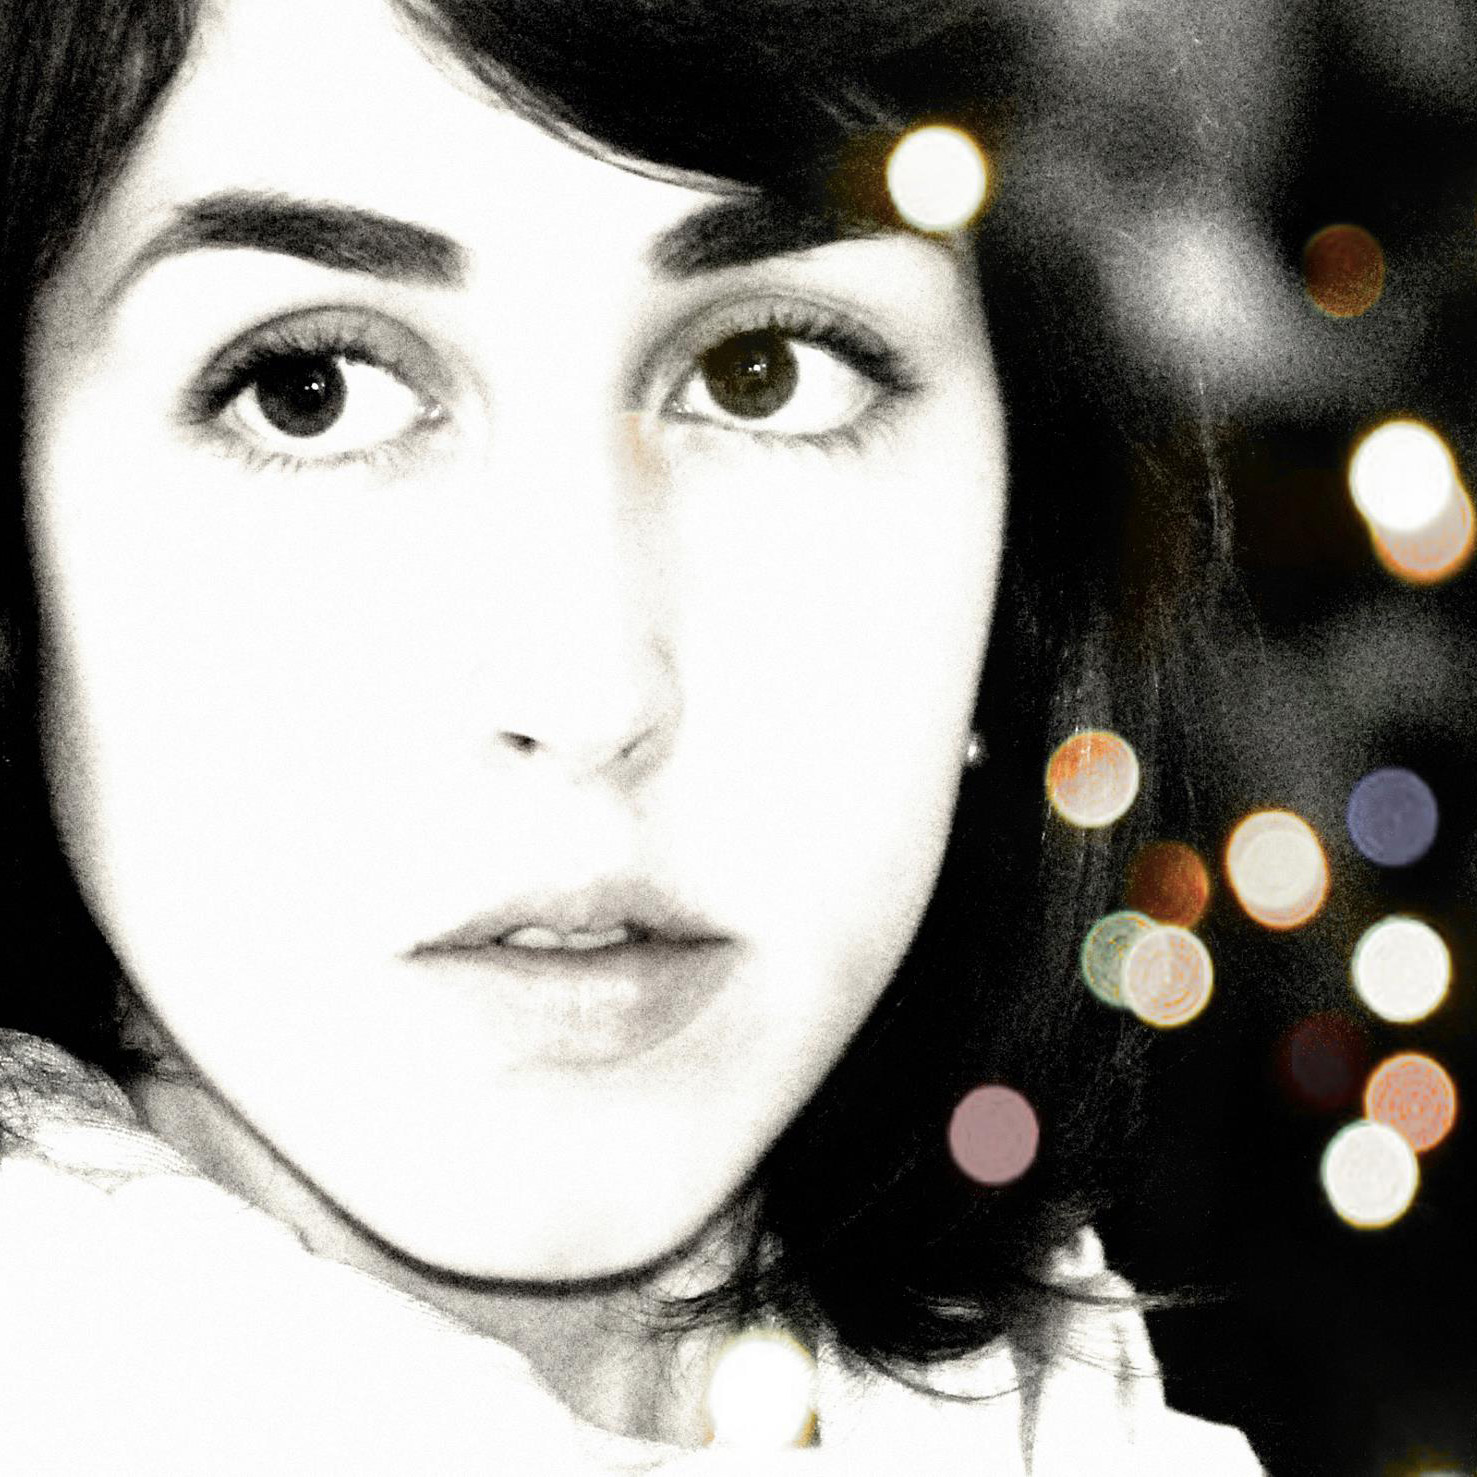
\includegraphics[width=.35\textheight]{gfx/saigethumb.jpg}
	 	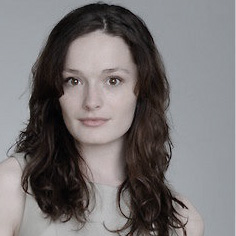
\includegraphics[width=.35\textheight]{gfx/genevievethumb.jpg}
	\end{center}


\clearpage

\section{What We Do}

\begin{enumerate}
	\item Improve computer science academics
	\item Schedule tutorials for lower level classes
	\item Game nights!
	\item Plan events
		\subitem Mini hackathons and programming workshops
		\subitem Barbecues and parties
		\subitem The "Awkward" events
\end{enumerate}

\clearpage

\section{New Stuff We Hope to Do}

\begin{itemize}
	\item Hardware workshop!!  Learn the basics of Arduino and some other hardware
	\item Organise research and student research talks
			\subitem - McGill is a massive research hub
			\subitem - Talk to Victor Chisholm, Nathan Friedman, \newline \space \hspace*{2.5em} or Calem Bendell about research opportunities
			\subitem - Think about it early!!
\end{itemize}

\clearpage

\section{Why Computer Science?  \\ Here's stuff \textit{undergraduates} have done}

\begin{itemize}
	\item Crunch biophysical or biochemical or economic or anthropological or social data and publish research papers
	\item Make new website to send directions to places over text
	\item Work towards a better home automation system
	\item Make a device to track back movement
	\item Automatically trade on foreign exchange markets
\end{itemize}

\clearpage


\section{HackMcGill}
\begin{multicols}{2}
	
\includegraphics[width=.45\textwidth]{gfx/HackMcGilllogo.png}
\begin{itemize}
	\item Organises most of the coding jams and helps get you to hackathons
	\item fb.com/groups/hackmcgill/
\end{itemize}
\end{multicols}
\clearpage


\section{Recruiting}

\begin{multicols}{2}
\begin{itemize}
	\item U1 Representative - Pick up Nomination form at Tr1060 (you'll get an email) (also Tr is the building we're sitting in)
	\item Make a rep role or come up with something awesome
\end{itemize}

\includegraphics[width=.4\textwidth]{gfx/darkside.jpg}
\end{multicols}

\clearpage

\section{Spam Us!}

\subsection{Facebook Groups}

https://www.facebook.com/groups/mcgillcsus/ \\
https://www.facebook.com/groups/mcgillcs/

\subsection{Github}

https://github.com/mcgill-csus \\
(don't know git?!  you will soon)

\clearpage

	
\end{document}